\chapter{Autoencoders}

Having introduced the basics of neural networks in chapter \ref{preliminary} we can consider a specific architecture of a neural network, a so called autoencoding neural network, or short: autoencoder. The idea of autoencoders is to take a given input, compress the input to a smaller size (usually called encoding) and afterwards, expand it as accurately as possible to the original size again (usually called decoding). Such an architecture is widely used in different applications. For example on social media platforms, where users send images to one another. Instead of sending the original image, which size might very well be a couple of megabytes, the image is firstly being encoded and sent in the compressed representation. Afterwards, the recipient decodes the image to its original representation. This way one has only to transmit the encoded representation, which usually is smaller by magnitudes.
Another very important application of autoencoders is in the machine learning field. Most state of the art machine learning models are using autoencoding structures, since it is way more efficient to first encode the data and then run a model on the encoded data. This is quite straight-forward, considering the same argument as in the previous use case - the encoded data being smaller by magnitudes. This way processing the samples can happen much faster compared to the non-encoded data samples and secondly, it makes storing data (on the drive and in memory) much more efficient.\\
In this chapter we want to consider how to formulate autoencoding neural networks from a mathematical point of view, take a look at some important results and lastly, analyse the theory in multiple applications using Python.

\section{Conceptional ideas}

As already mentioned, an autoencoding neural network first compresses/encodes the input data to a smaller representation. The size of this smaller representation is usually referred to as bottleneck of the autoencoder. afterwards, the autoencoding neural network expands/decodes the data to its original size. Hence, we can divide these two steps into separate architectures - the encoding and the decoding part of the neural network, which we will formulate separately. In figure \ref{autoencoder} we can take a look at a visual example of an autoencoding architecture.\\
One should mention, that since the goal of an autoencoding neural network ultimately is to alter and reconstruct images, we approach this in an unsupervised learning setting. Hence, we compare the output of the neural network to the input. This forces us to consider slightly different loss functions.


\begin{definition}
Let $X, Y$ be Banach spaces representing the input and output space, respectively.\\
Then a continuous function defined as
\begin{align*}
L:X\times Y &\to \R,\\
\left(x, p(x)\right) &\mapsto L(x, p(x)),
\end{align*}
is called \textbf{unsupervised loss function}.
\end{definition}


There are multiple important loss functions in the computer vision setting. We will consider a couple of those in the following example. For further reading please take a look at \cite{foster2022generative}


\begin{example}
Let $\O$ be a pixel domain with resolution $(M,N)$ and $d$ the number of channels. Furthermore, let $f$ be a neural network with arbitrary but fixed architecture.\\
Then the following functions are loss functions operating on images.
\begin{mydescription}{\widthof{\textbf{Binary Cross-Entropy (BCE)}}}
\item[\textbf{Mean Squared Error (MSE)}] \begin{align*}
\MSE(\p, f(\p)) = \sum_{i=1}^{M}\sum_{j=1}^{N}\left\|\p_{ij} - f(\p)_{ij}\right\|^2,
\end{align*}
\item[\textbf{Binary Cross-Entropy (BCE)}]
\begin{align*}
\BCE(\p, f(\p)) = - \frac{1}{MN}\sum_{i=1}^{M}\sum_{j=1}^{N} \biggl(&\p_{ij} \log\left(f\left(\p\right)_{ij}\right)\\ + \bigl(1-&\p_{ij}\bigr)\log\left(1 - f\left(\p\right)_{ij}\right)\biggr),
\end{align*}
\end{mydescription}
where $\p$ denotes an image defined on $\P_{\O}$.
\end{example}


\begin{remark}
The Binary Cross-Entropy loss function is usually used for binary classification problems. However, it still works in computer vision.
\end{remark}


\begin{figure}[H]
\begin{center}
   \begin{minipage}[b]{0.9\linewidth}
      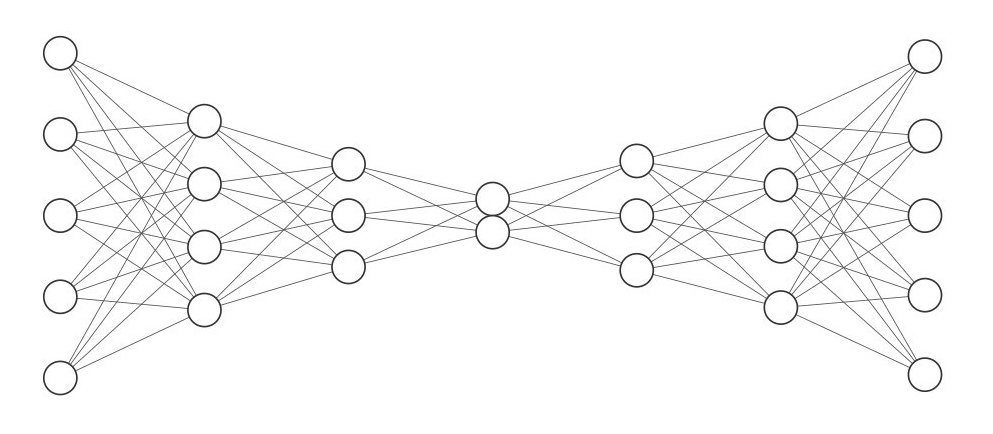
\includegraphics[width=\linewidth]{autoencoder}
      \caption{An autoencoding neural network with input and output $x, y\in \R^5$. The five hidden layers have dimensions $4$, $3$, $2$, $3$ and $4$ respectively. Hence, the bottleneck dimension is $2$ in this example. The graphic was generated with http://alexlenail.me/NN-SVG/index.html}\label{autoencoder}
	\end{minipage}
\end{center}
\end{figure}


If we divide the autoencoder as described above, we firstly obtain the encoder as we can see in figure \ref{img_encoder} or formally defined as follows.

\begin{definition}\label{def_encoder}
Let $\T$ be a parameter space and $\t \in \T$ a set of parameters, $L\in \N$ and $d_1,\ldots, d_L\in\N$. Let further $\f$ be an activation function and $f_{\f,L,\t}$ a neural network.\\
If the neural network $f_{\f,L,\t}$ fulfils the condition $n_i= d_1 \geq \ldots \geq d_L = n_o$ with $n_i, n_o \in \N$ being the input and output dimensions respectively, then we speak of an \textbf{encoding neural network} (or short: \textbf{encoder}) and denote it as $f_e$.
\end{definition}


\begin{figure}[H]
\begin{center}
   \begin{minipage}[b]{0.9\linewidth}
      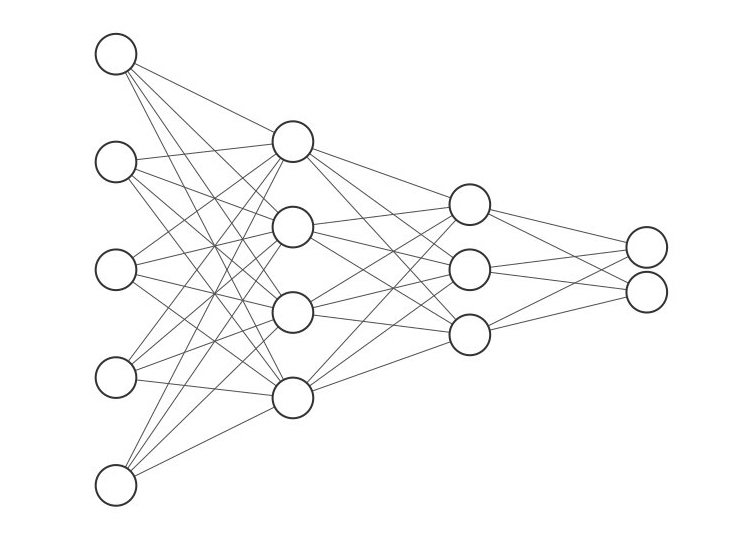
\includegraphics[width=\linewidth]{encoder}
      \caption{An encoding neural network with input $x\in \R^5$ and output $y \in \R^2$. The two hidden layers have dimensions $4$ and $3$. Hence, the encoder reduces the data dimensionality from $5$ to $2$ dimension. The graphic was generated with http://alexlenail.me/NN-SVG/index.html}\label{img_encoder}
	\end{minipage}
\end{center}
\end{figure}


For the second part of the divided autoencoding structure, we obtain the decoder as we can see in figure \ref{img_decoder}. We can define this architecture analogously to the encoder in definition \ref{def_encoder}.


\begin{definition}\label{def_decoder}
Let $\T$ be a parameter space and $\t \in \T$ a parameter, $L\in \N$ and $d_1,\ldots, d_L\in\N$. Let further $\f$ be an activation function and $f_{\f,L,\t}$ a neural network.\\
If the neural network $f_{\f,L,\t}$ fulfils the condition $n_i= d_1 \leq \ldots \leq d_L = n_o$ with $n_i, n_o \in \N$ being the input and output dimensions respectively, then we speak of an \textbf{decoding neural network} (or short: \textbf{decoder}).
\end{definition}


\begin{figure}[H]
\begin{center}
   \begin{minipage}[b]{0.9\linewidth}
      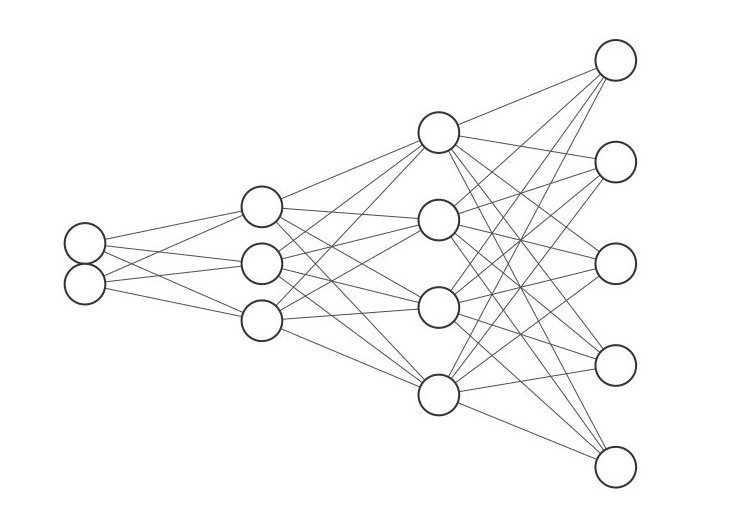
\includegraphics[width=\linewidth]{decoder}
      \caption{A decoding neural network with input $x\in \R^2$ and output $y \in \R^5$. The two hidden layers have dimensions $3$ and $4$. Hence, the decoder expands the data dimensionality from $2$ to $5$ dimensions. The graphic was generated with http://alexlenail.me/NN-SVG/index.html}\label{img_decoder}
	\end{minipage}
\end{center}
\end{figure}

Before combining the encoding and the decoding structure to obtain the autoencoding neural network, we need to consider the following technicality first.

\begin{lemma}
Let $f_1, f_2$ be two neural networks of depths $L_1, L_2 \in \N$ with parameters $\t_1, \t_2 \in \T$, where $\T$ is an arbitrary parameter space. Furthermore, let the dimensions of each layer be $d_1, \ldots, d_{L_1} \in \N$ of $f_1$ and $\tilde{d}_1, \ldots, \tilde{d}_{L_2} \in \N$ of $f_2$. Additionally, let $d_{L_1} = \tilde{d}_1$.\\
Then their composition $f_2\circ f_1$ is a neural network of depth $L_1 + L_2$ with parameters $(\t_1, \t_2)$.
\end{lemma}

\begin{proof}
Since $f_1$ is a neural network of depth $L_1$ with parameters $\t_1$, its architecture looks like
\begin{align}\label{nn_1}
f_1 (x) = H_{L_1} \circ H_{L_1-1} \circ \ldots H_{2} \circ H_1 (x),\qquad x \in \R^{d_1}.
\end{align}
Analogously, we can write $f_2$ as
\begin{align}\label{nn_2}
f_2 (y) = \tilde{H}_{L_2} \circ \tilde{H}_{L_2-1} \circ \ldots \tilde{H}_{2} \circ \tilde{H}_1 (y), \qquad y \in \R^{\tilde{d}_1}.
\end{align}
Since we assumed that the output dimension $d_{L_1}$ of the neural network $f_1$ is equal to the input dimension $\tilde{d}_1$ of the neural network $f_2$, we can consider the result of \eqref{nn_1} as input for \eqref{nn_2}
\begin{align*}
y &\coloneqq H_{L_1} \circ H_{L_1-1} \circ \ldots H_{2} \circ H_1 (x), \qquad x \in \R^{d_1}.
\end{align*}
Hence, we obtain
\begin{align}\label{nn_comp}
f_2 (y) &= \tilde{H}_{L_2} \circ \tilde{H}_{L_2-1} \circ \ldots H_{2} \circ \tilde{H}_1 (y),\nonumber\\
f_2\left(f_1\left(x\right)\right)  &= \tilde{H}_{L_2} \circ \tilde{H}_{L_2-1} \circ \ldots H_{2} \circ \tilde{H}_1 \left( H_{L_1} \circ H_{L_1-1} \circ \ldots H_{2} \circ H_1 (x) \right),\nonumber\\
f_2\left(f_1\left(x\right)\right)  &= \tilde{H}_{L_2} \circ \tilde{H}_{L_2-1} \circ \ldots H_{2} \circ \tilde{H}_1 \circ H_{L_1} \circ H_{L_1-1} \circ \ldots H_{2} \circ H_1 (x), \qquad x \in \R^{d_1}.
\end{align}
Hence, the composition $f_2 \circ f_1$ is a neural network of depth $L_1 + L_2$, what follows from \eqref{nn_comp}.\\
Lastly, we consider the parameters $\t$ of the neural network $f_2 \circ f_1$. Since the parameters of a neural network were defined as $\t = (\t_1,\ldots, \t_L)$, where each entry is defined as $\t_i = (W_i, b_i)$ and denotes the weight and bias of each layer $H_i$ or $\tilde{H}_i$, respectively, we can write the parameters of both neural networks as
\begin{align*}
\t_1 &\coloneqq (\t_1, \ldots, \t_{L_1}) = \left((W_1, b_1),\ldots, (W_{L_1}, b_{L_1}) \right),\\
\t_2 &\coloneqq (\tilde{\t}_1, \ldots, \tilde{\t}_{L_2}) = \left((\tilde{W}_1, \tilde{b}_1),\ldots, (\tilde{W}_{L_2}, \tilde{b}_{L_2}) \right).
\end{align*}
Hence, the composition $f_2\circ f_1$ has the parameters
\begin{align*}
\t  &= \left((W_1, b_1),\ldots, (W_{L_1}, b_{L_1}), (\tilde{W}_1, \tilde{b}_1),\ldots, (\tilde{W}_{L_2}, \tilde{b}_{L_2})  \right)\\
&= \left(\t_1,\ldots \t_{L_1}, \tilde{\t}_1, \ldots, \tilde{\t}_{L_2} \right) \eqqcolon \left(\t_1,\t_2 \right).
\end{align*}
\end{proof}

\begin{definition}\label{def_autoencoder}
Let $f_e$ and $f_d$ be an encoding and a decoding neural network with input dimension $n_i$ in $\N$ and output of the encoding neural network $n_b$ in $\N$, that we will refer to as \textbf{bottleneck} of the autoencoding neural network.
Then we define an \textbf{autoencoding neural network} $f_a$ as the composition
\begin{align*}
f_a: \R^{n_i} &\to \R^{n_i},\\
x &\mapsto \left(f_d \circ f_e \right)(x).
\end{align*}
\end{definition}
